\documentclass{article}

\usepackage{graphicx}
\usepackage{float}
\usepackage{listings}
\usepackage{indentfirst}
\usepackage[a4paper, total={6in, 8in}]{geometry}
\usepackage{hyperref}
\usepackage{fancyhdr}
\usepackage{xepersian}
\settextfont{B Nazanin}
\setlatintextfont{Times New Roman}

\begin{document}


%title page%
\begin{titlepage}
	\begin{center}
		\textbf{ \Huge{به نام خدا}}
	
		\vspace{0.2cm}
		
		
\includegraphics[width=0.4\textwidth]{sharif.png}\\
		\vspace{0.2cm}
		\textbf{ \Huge{آزمایش شماره 6}}\\
		\vspace{0.25cm}
		\textbf{ \Large{آز معماری - دکتر سربازی آزاد}}
		\vspace{0.2cm}
		
		
		\large \textbf{دانشکده مهندسی کامپیوتر}\\\vspace{0.1cm}
		\large   دانشگاه صنعتی شریف\\\vspace{0.2cm}
		\large   ﻧﯿﻢ‌سال اول ۰۰-۰۱ \\\vspace{0.10cm}
		\large{گروه:}\\
		\large{\href{mailto:a.h.hadian@gmail.com}{امیرحسین هادیان - ۹۷۱۰۲۶۰۹}}\\
		\large{\href{mailto:mofayezi.m@gmail.com}{محمدرضا مفیضی - ۹۸۱۰۶۰۵۹}}\\
		\large{\href{mailto:a.hatam008@gmail.com}{علی حاتمی تاجیک - ۹۸۱۰۱۳۸۵}}\\
	\end{center}
\end{titlepage}
%title page%

\newpage

%pages header
\pagestyle{fancy}
\fancyhf{}
\fancyfoot{}
\setlength{\headheight}{59pt}
\cfoot{\thepage}
\lhead{آزمایش شماره 6}
\rhead{
\includegraphics[width=0.1\textwidth]{sharif.png}\\
		دانشکده مهندسی کامپیوتر
}
\chead{آز معماری}
%pages header

\section{هدف}
هدف از انجام این آزمایش متصل کردن بخش محاسبات طراحی شده در بخش قبل به یک حافظه برنامه‌پذیر است که برنامه محاسبه عدد دهم دبناله فیبوناچی است.

\section{طراحی}
این بخش نیاز به طراحی خاصی نداشت چرا که از همان مدار آزمایش قبل استفاده شده است با این تفاوت که دیگر دستورات را به صورت دستی وارد نمی‌کنیم و از یک حافظه‌ برنامه‌پذیر برای دادن برنامه به آن استفاده می‌کنیم. در این قسمت دو بخش اصلی داریم: اول، ساخت یک شمارنده ۵ بیتی و دوم، نوشتن برنامه مورد نظر به صورتی که بتوان آنرا در \lr{EPROM} نوشت.

\subsection{شمارنده ۵ بیتی}
با استفاده از طراحی که در درس مدارهای‌ منطقی برای شمارنده انجام داده‌ایم استفاده می‌کنیم و برای اختصار توضیح زیادی درباره آن نمی‌دهیم. این شمارنده یک شمارنده ۵ بیتی آسنکرون است که با استفاده از پنج فلیپ‌فلاپ \lr{JK} ساخته شده است. شماتیک این شمارنده در شکل \ref{counter} آمده است.

\begin{figure}[H]
	\centering
	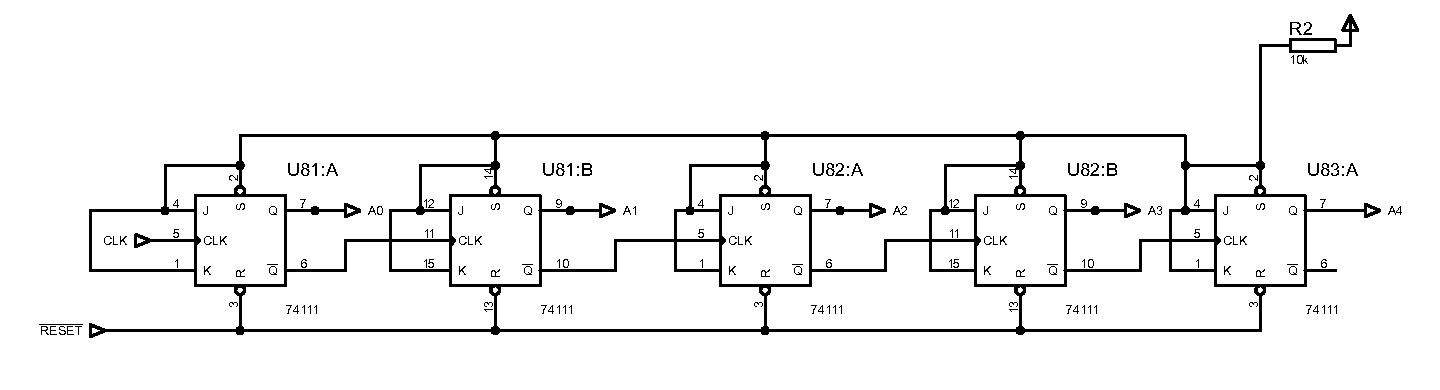
\includegraphics[scale=0.5]{./graphics/counter}
	\caption{شمارنده پنج بیتی}
	\label{counter}
\end{figure}

\subsection{نوشتن برنامه}
ابتدا با توجه به صورت دستور در آزمایش قبل کد را به زبان ماشین ترجمه می‌کنیم:

\begin{table}[H]
\centering
\begin{latin}
\begin{tabular}{|l|l|l|l|}
\hline
\multicolumn{1}{|c|}{\textbf{Address}} & \multicolumn{1}{c|}{\textbf{Binary Code}} & \multicolumn{1}{c|}{\textbf{Hex Code}} & \multicolumn{1}{c|}{\textbf{Code}} \\ \hline
00000 & 00 1 00 000 & 20 & SUB R0,R0 \\ \hline
00001 & 00 0 01 101 & 0D & ADD R1,1  \\ \hline
00010 & 00 0 00 001 & 01 & ADD R0,R1 \\ \hline
00011 & 00 0 01 001 & 09 & ADD R1,R0 \\ \hline
00100 & 00 0 00 001 & 01 & ADD R0,R1 \\ \hline
00101 & 00 0 01 001 & 09 & ADD R1,R0 \\ \hline
00110 & 00 0 00 001 & 01 & ADD R0,R1 \\ \hline
00111 & 00 0 01 001 & 09 & ADD R1,R0 \\ \hline
01000 & 00 0 00 001 & 01 & ADD R0,R1 \\ \hline
01001 & 00 0 01 001 & 09 & ADD R1,R0 \\ \hline
\end{tabular}
\end{latin}
\caption{کد مربوط به تولید عدد دهم فیبوناچی}
\label{tab:codes}
\end{table}

سپس با استفاده از نرم‌افزار \lr{HxD} این کد هگزادسیمال ساخته شده را به صورت یک فایل هگر ۱۶ بیتی می‌نویسیم (این فایل یک نوع فایل متنی است که در ابتدای هر خط به فرمت خاصی عبارات نوشته می‌شوند و قابل استفاده برای شبیه سازی \lr{EPROM} در پروتئوس خواهد بود. این فایل دارای محتویات زیر است که کد هگز ما درون آن مشخص است:

\begin{latin}
\begin{lstlisting}
:0A000000200D0109010901090109A1
:00000001FF
\end{lstlisting}
\end{latin}

\subsection{مدار نهایی}
با اتصال شمارنده به حافظه برنامه‌پذیر و دادن برنامه به آن، خروجی‌های حافظه را به عنوان خطوط کنترلی واحد محاسبات که در آزمایش قبل ساخته بودیم استفاده می‌کنیم. شکل  نشان‌دهنده مدار نهایی است.

برای راحتی کار و اینکه نیازی نباشد تا برای هر دستور دکمه کلاک را فشار دهیم، از این ساز و کار استفاده می‌کنیم که با استفاده از یک گیت \lr{OR} معکوس عدد ۱۰ (شماره برنامه‌ای که دیگر نباید اجرا شود) را با سیگنال کلاک \lr{AND} می‌کنیم تا پس از آن کلاک به سیستم اعمال نشود و عملا سیستم در حالت \lr{Idle} قرار بگیرد. شکل \ref{main} نشان‌دهنده شمای کلی مدار است.

\begin{figure}[H]
	\centering
	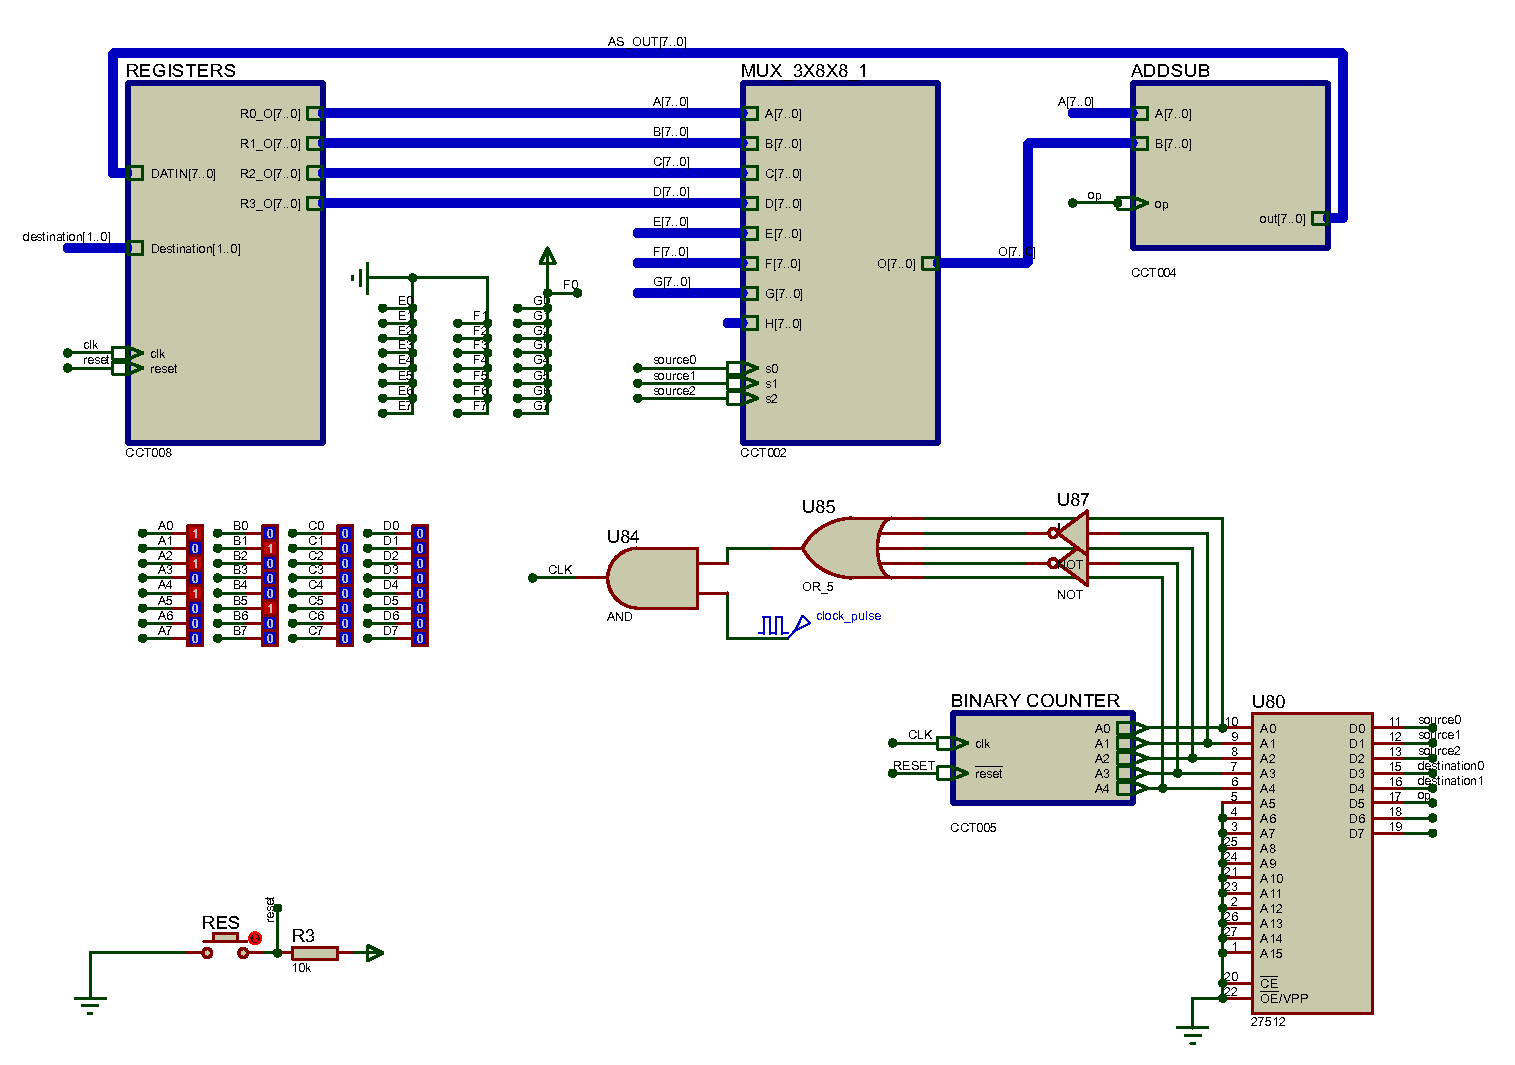
\includegraphics[scale=0.5]{./graphics/main}
	\caption{مدار اصلی}
	\label{main}
\end{figure}

\section{تست}
نتیجه اجرای کد در شکل \ref{main} آمده است و واضح است که عدد ۳۴ درون رجیستر شماره ۱ وجود دارد. (رجیستر شماره ۰ حامل عدد ۲۱ است)

\end{document}
